% This file was generated with po4a. Translate the source file.
%
\pdfobjcompresslevel=1 \documentclass[notes=hide]{beamer}
\usetheme[titlepagelogo=img2/cover]{LDN}

\usepackage[utf8]{inputenc}
\usepackage[francais]{babel}
\usepackage[T1]{fontenc}
\usepackage{tabularx, verbatim, xcolor, textpos}
\usepackage{lmodern, alltt, graphicx, ragged2e}
\usepackage{marvosym, multicol, textcomp, eurosym}

\definecolor{darkgreen}{RGB}{0,99,0}
\newcommand{\good}{{\color{green}\Smiley}}
\newcommand{\bad}{{\color{red}\Frowny}}
\colorlet{titre}{white} \setbeamercolor{normal text}{fg=white,bg=white}

\date{\textbf{AG FFDN 2015}}

\title{Internet³}
\subtitle{\vspace{10pt}\emph{Neutral Internet \& Self-hosting}}
\author{Neutrinet \\ Lorraine Data Network \\ YunoHost}
\begin{document}

\begin{frame}[t,plain]
\titlepage
  \begin{textblock}{}(10,-7)
    
\includegraphics[height=1.5cm]{img2/logo-ynh-black.pdf}
  \end{textblock}
  \begin{textblock}{}(9.5,-4)
    \includegraphics[height=1.2cm]{img2/logoldn}
  \end{textblock}
  \begin{textblock}{}(10,-1.5)
    
\includegraphics[height=1.5cm]{img2/logo-neutrinet}
  \end{textblock}\color{black}\textbf{OuiShareLabs May 2015}
\end{frame}

\watermarkon \watermarkoff

\setbeamercolor{background canvas}{bg=black}
\begin{frame}[t,plain]
\begin{center}
  \vspace{\fill}

\includegraphics[width=230pt]{img2/ffdn.png}
  \vspace{\fill}
  \color{white}{\fontsize{30}{30}\selectfont Fédération FDN}
\end{center}
\end{frame}

\begin{frame}[t,plain]
  \begin{center}
    \vspace{\fill}
      \color{white}{\fontsize{60}{60}\selectfont libre, neutral}
    \vspace{\fill}
  \end{center}
\end{frame}

\begin{frame}[t,plain]
  \begin{center}
    \vspace{\fill}
      \color{white}{\fontsize{60}{60}\selectfont and decentralized}
    \vspace{\fill}
  \end{center}
\end{frame}

\begin{frame}[t,plain]
  \begin{center}
    \vspace{\fill}
      \color{white}{\fontsize{40}{40}\selectfont Libre \& neutral~?}
    \vspace{\fill}
  \end{center}
\end{frame}

\begin{frame}[t]
\frametitle{\textcolor{titre}{Whithout Internet³}}
  \color{red!60} \begin{center}

\includegraphics[width=0.9\textwidth]{img2/connexion1en.png}
  \end{center}
\end{frame}

\begin{frame}[t]
\frametitle{\textcolor{titre}{Whithout Internet³}}
  \begin{center}
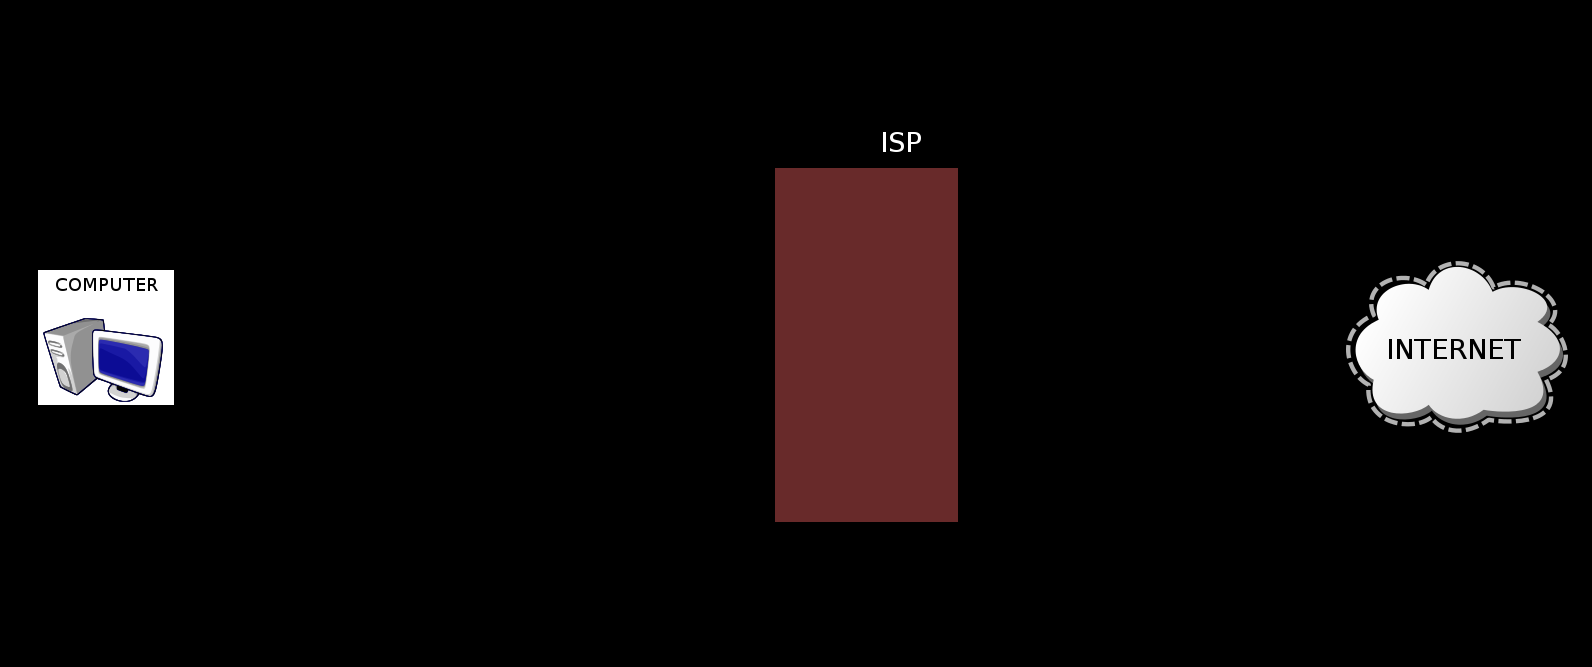
\includegraphics[width=0.9\textwidth]{img2/connexion2en.png}
  \end{center}
\end{frame}

\begin{frame}[t]
\frametitle{\textcolor{titre}{Whithout Internet³}}
  \begin{center}
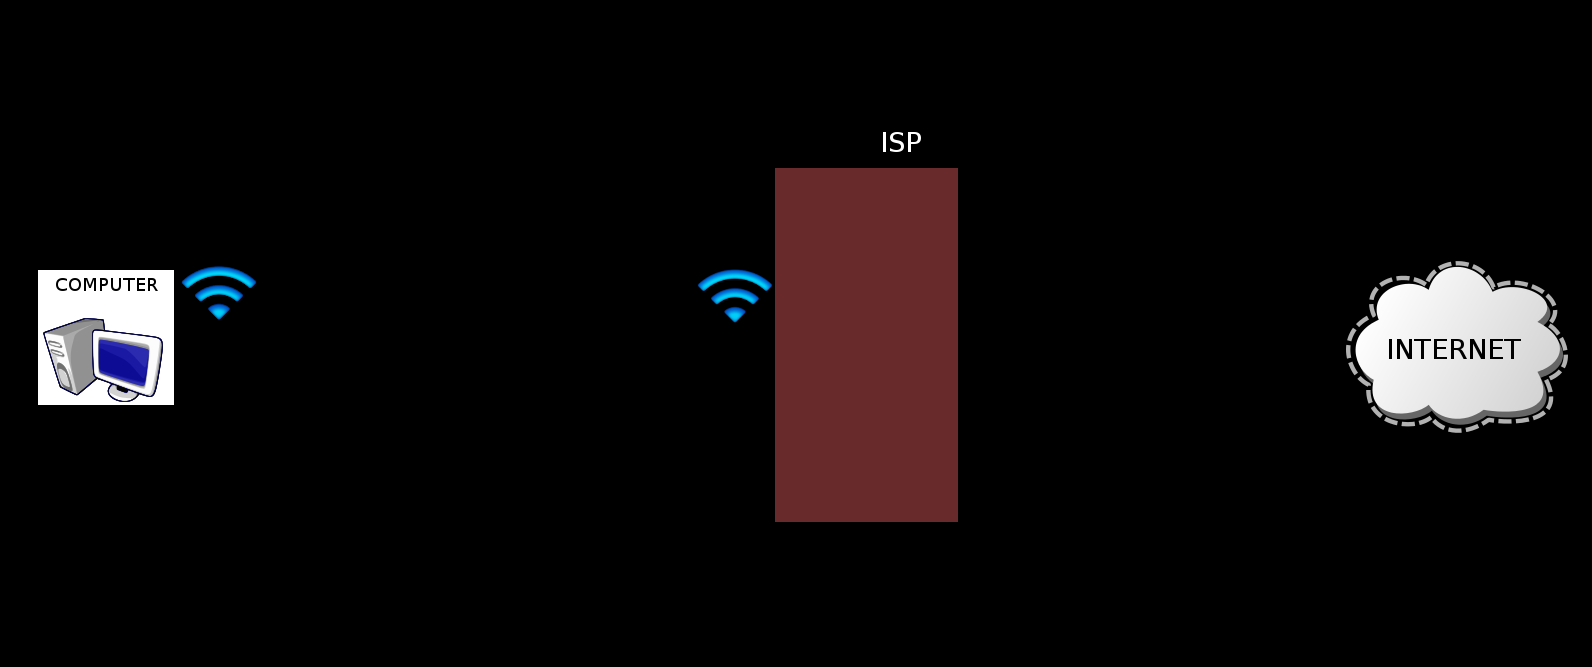
\includegraphics[width=0.9\textwidth]{img2/connexion3en.png}
  \end{center}
\end{frame}

\begin{frame}[t]
\frametitle{\textcolor{titre}{Whithout Internet³}}
  \begin{center}
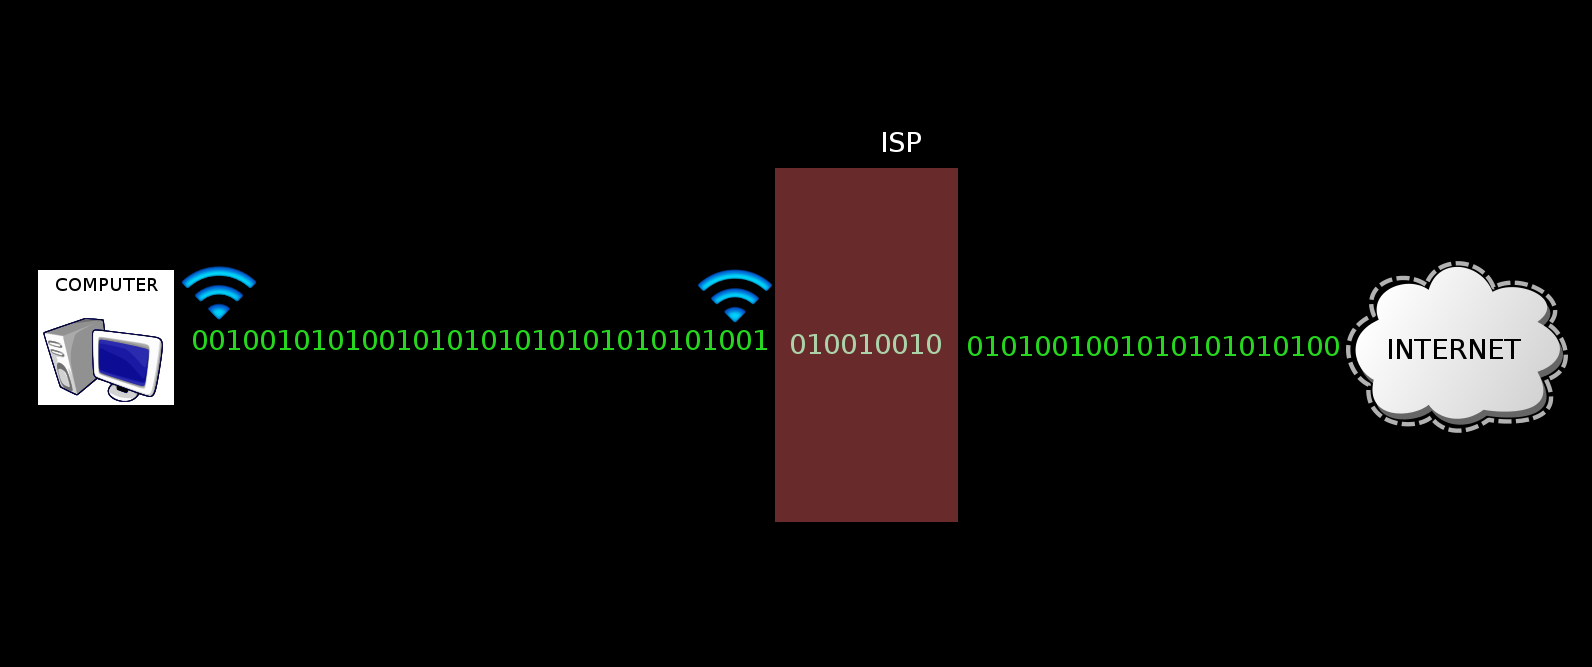
\includegraphics[width=0.9\textwidth]{img2/connexion4en.png}
  \end{center}
\end{frame}

\begin{frame}[t]
\frametitle{\textcolor{titre}{Problems ~?}}
  \begin{center}
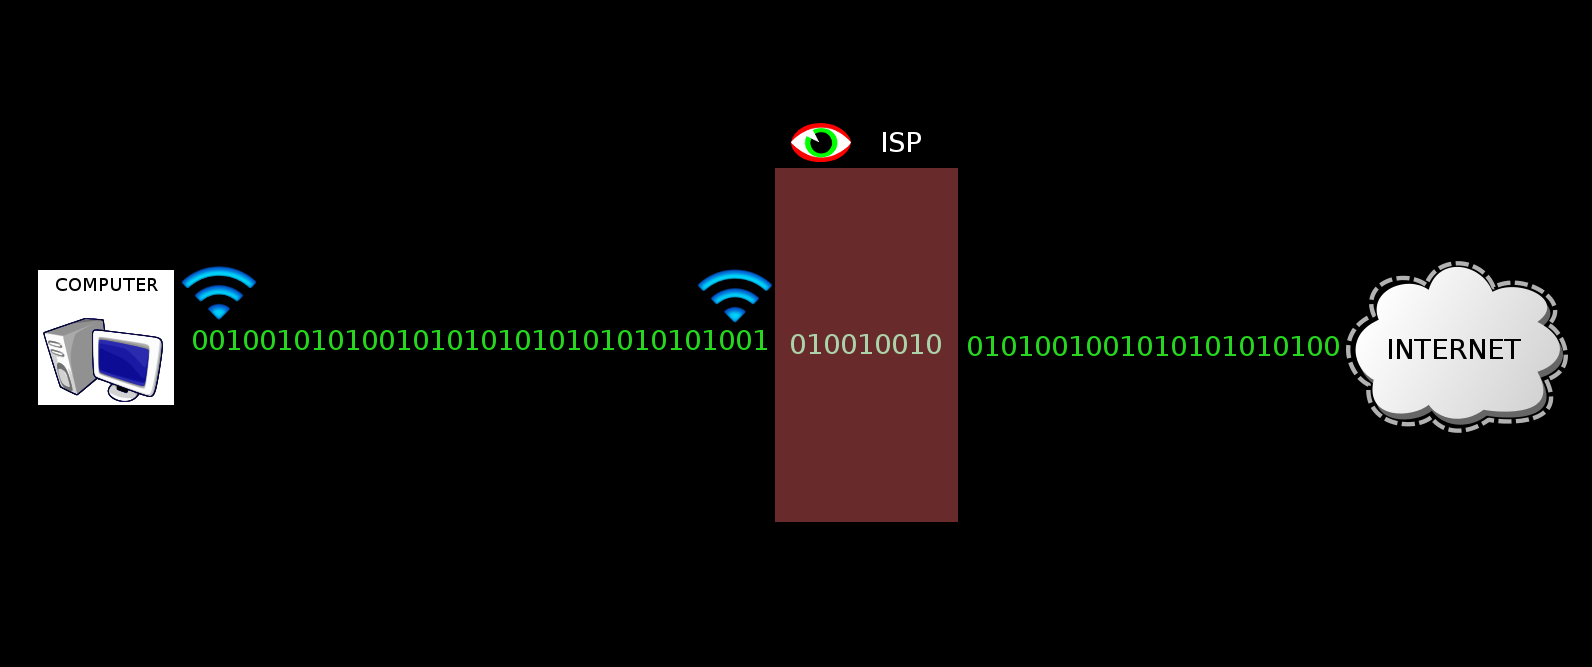
\includegraphics[width=0.9\textwidth]{img2/connexion5en.png}
  \end{center}
\end{frame}

\begin{frame}
\frametitle{\textcolor{titre}{Problems}}
  \begin{itemize}
    \item Traffic shaping (Comcast Vs Netflix)\pause
    \item Port blocking (port 25) \pause
    \item Dynamic IP addressing / no IPv6 \pause
    \item Censorship (DNS hijacking) \pause
    \item Surveillance (NSA/French Gov?)  \pause
    \item Use of personal data\pause
  \end{itemize}
\end{frame}

%\begin{frame}[t]
%		  \frametitle{\textcolor{titre}{Oath to NOT respect my privacy}}
%\begin{center}
%\vfill
%\includegraphics[width=.75\textwidth]{img2/03g-cgu.png}
%\vfill
%\end{center}
%\end{frame}

\begin{frame}[t]
\frametitle{\textcolor{titre}{With the Internet³}}
		  \color{red!60} \begin{center}
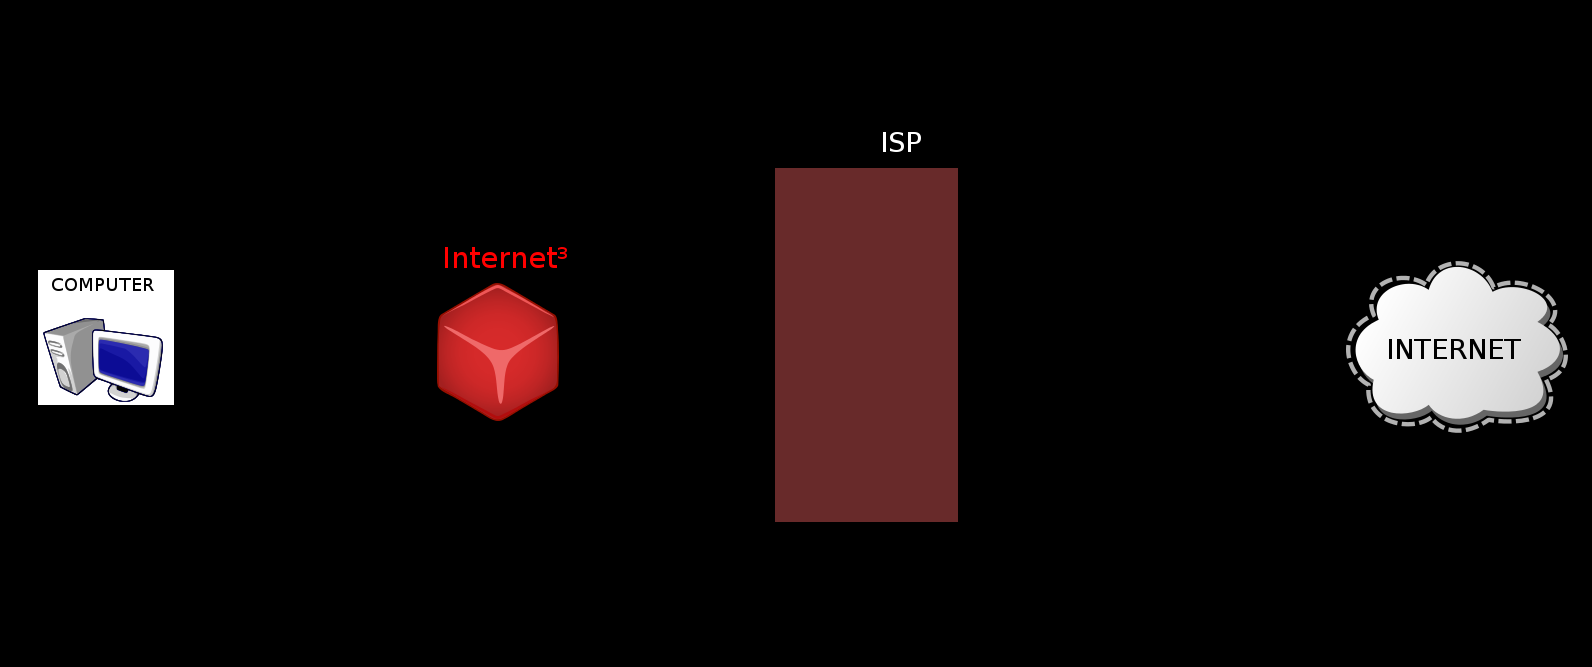
\includegraphics[width=0.9\textwidth]{img2/connexion11en.png}
		  \end{center}
\end{frame}
\begin{frame}[t]
\frametitle{\textcolor{titre}{With the Internet³}}
		  \begin{center}
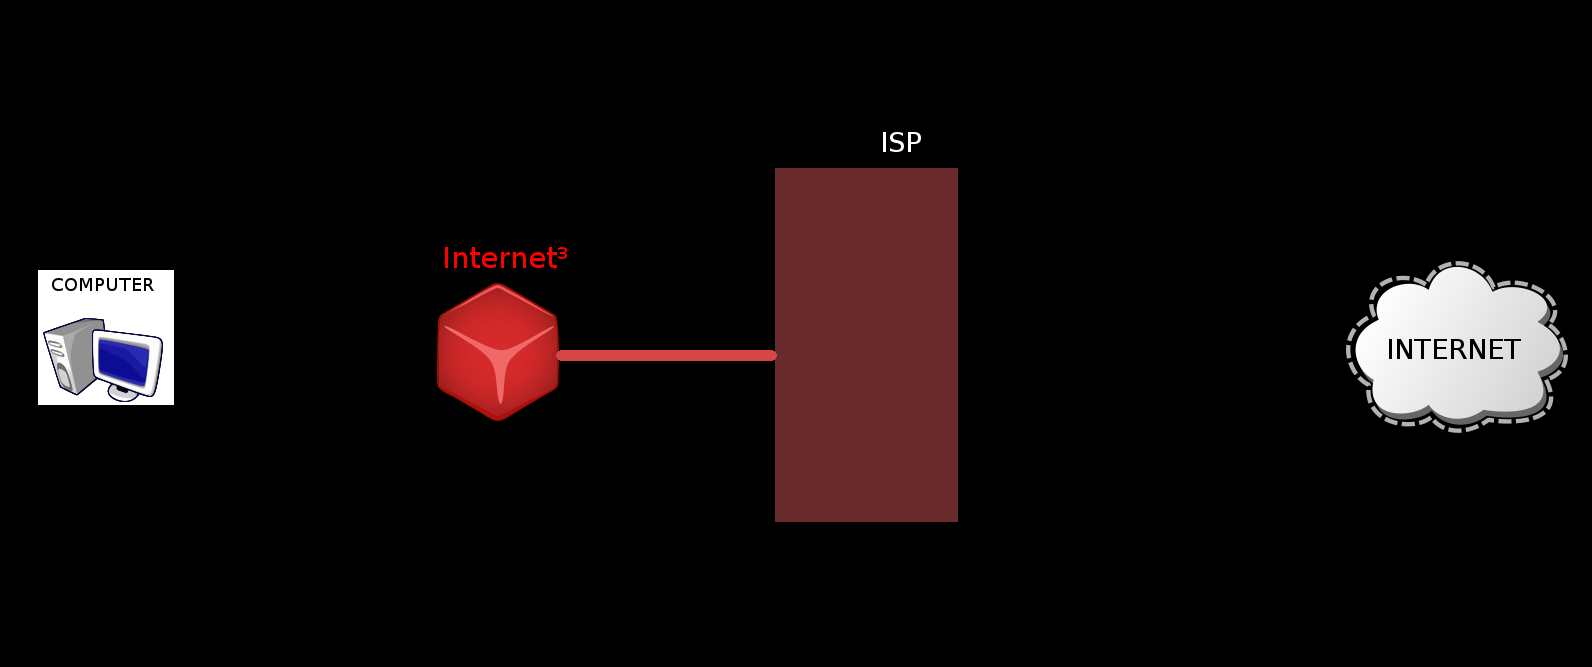
\includegraphics[width=0.9\textwidth]{img2/connexion12en.png}
		  \end{center}
\end{frame}
\begin{frame}[t]
\frametitle{\textcolor{titre}{With the Internet³}}
		  \begin{center}
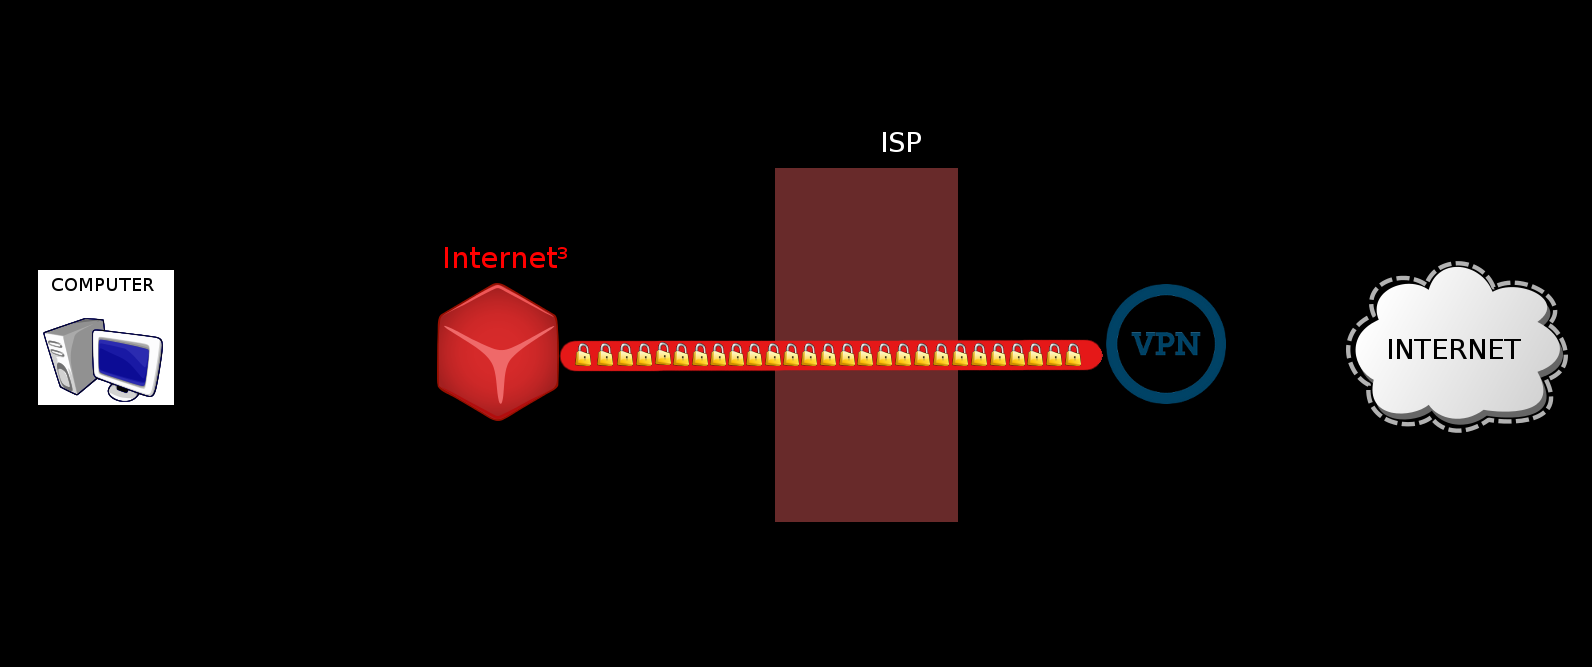
\includegraphics[width=0.9\textwidth]{img2/connexion13en.png}
		  \end{center}
\end{frame}
\begin{frame}[t]
\frametitle{\textcolor{titre}{With the Internet³}}
		  \begin{center}
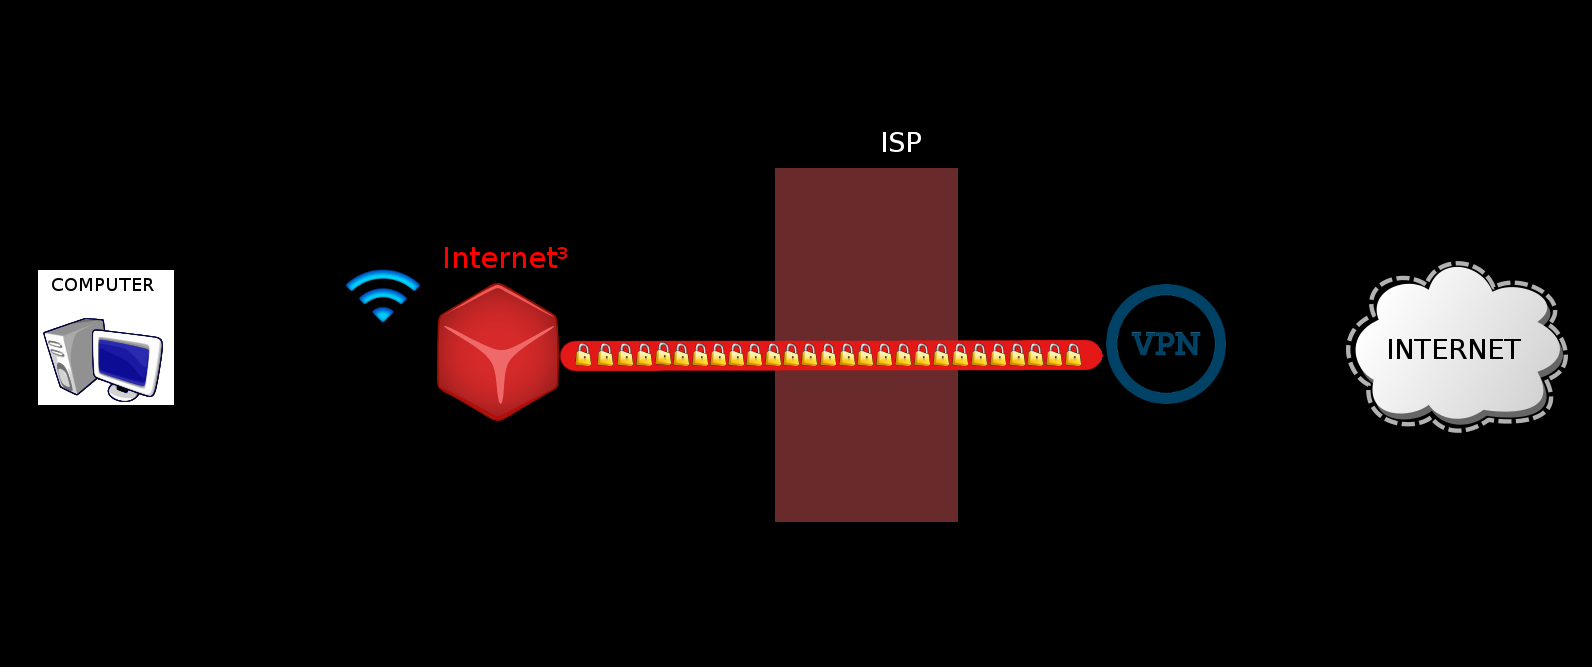
\includegraphics[width=0.9\textwidth]{img2/connexion14en.png}
		  \end{center}
\end{frame}

\begin{frame}[t]
		  \frametitle{\textcolor{titre}{With the Internet³}}
		  \begin{center}
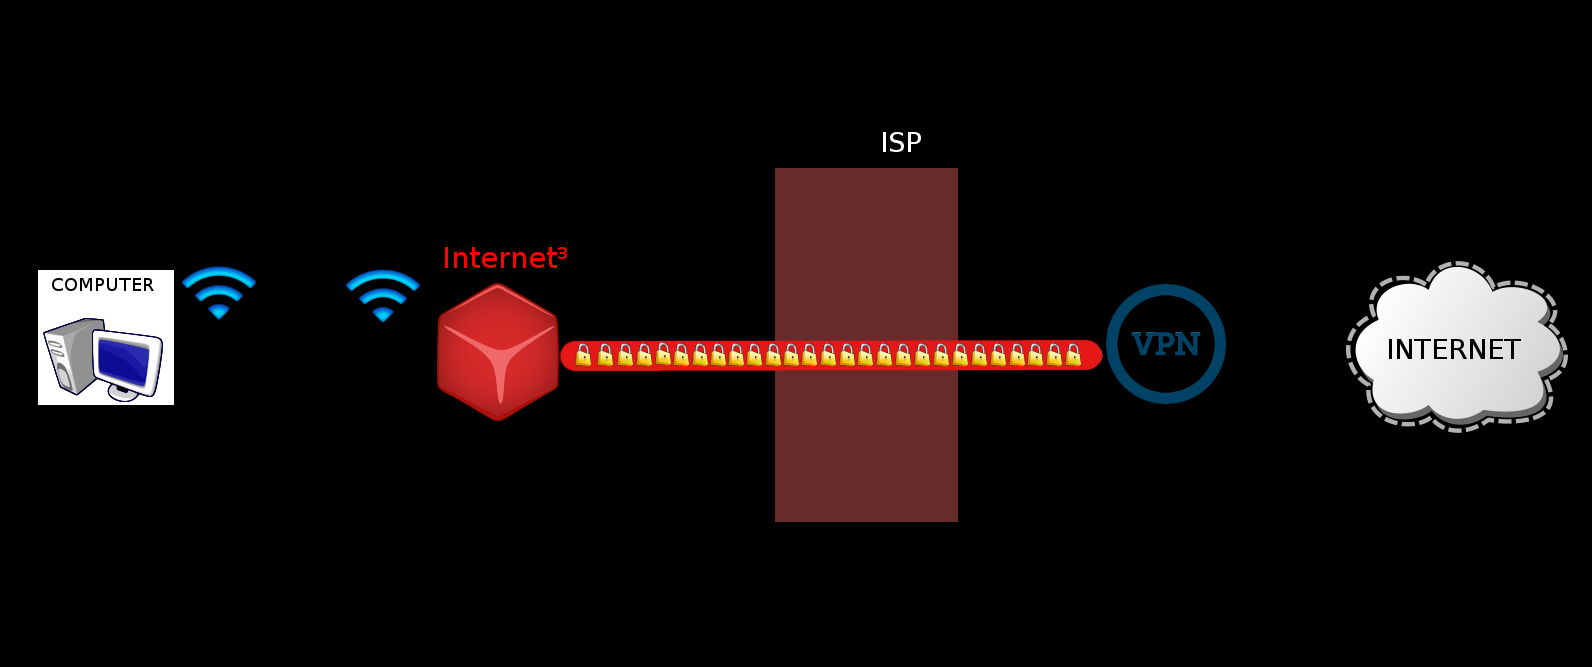
\includegraphics[width=0.9\textwidth]{img2/connexion15en.png}
		  \end{center}
\end{frame}


\begin{frame}[t]
		  \frametitle{\textcolor{titre}{With the Internet³}}
		  \begin{center}
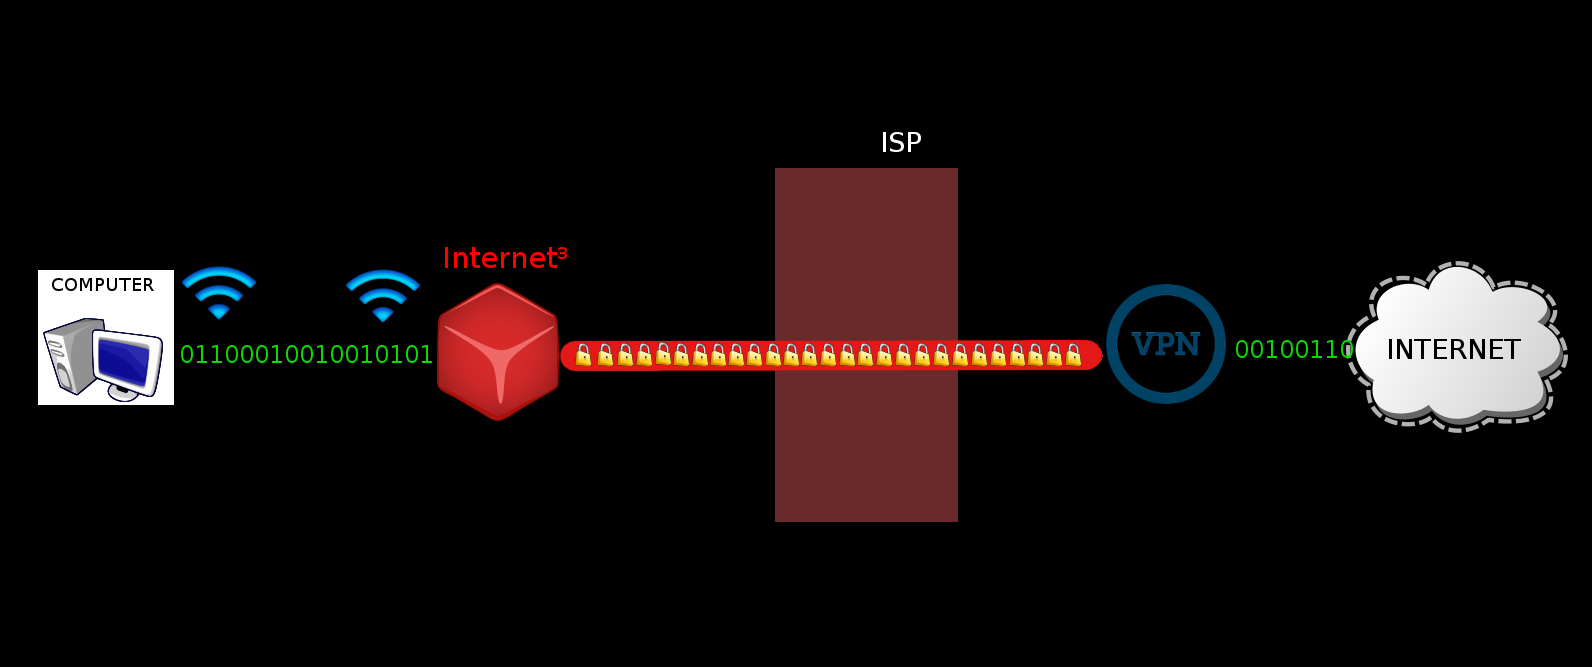
\includegraphics[width=0.9\textwidth]{img2/connexion16en.png}
		  \end{center}
\end{frame}

\begin{frame}
		  \frametitle{\textcolor{titre}{Problems ~?}}
					 \begin{itemize}
								\item Traffic shaping (Comcast Vs Netflix)  
								\item Port blocking (port 25) 
								\item Dynamic IP addressing / no IPv6 
								\item Censorship (DNS hijacking) 
								\item Surveillance (NSA/French Gov?)  
								\item Use of personal data 
					\end{itemize}
\end{frame}

\begin{frame}
		  \frametitle{\textcolor{titre}{Problems ~?}}
					 \begin{itemize}
								\item
								\item Port blocking (port 25) 
								\item Dynamic IP addressing / no IPv6 
								\item Censorship (DNS hijacking) 
								\item Surveillance (NSA/French Gov?)  
								\item Use of personal data 
					\end{itemize}
\end{frame}

\begin{frame}
		  \frametitle{\textcolor{titre}{Problems ~?}}
					 \begin{itemize}
								\item
								\item
								\item Dynamic IP addressing / no IPv6 
								\item Censorship (DNS hijacking) 
								\item Surveillance (NSA/French Gov?)  
								\item Use of personal data 
					\end{itemize}
\end{frame}





\begin{frame}
		  \frametitle{\textcolor{titre}{Problems ~?}}
					 \begin{itemize}
								\item
								\item
								\item
								\item Censorship (DNS hijacking) 
								\item Surveillance (NSA/French Gov?)  
								\item Use of personal data 
					\end{itemize}
\end{frame}

\begin{frame}
		  \frametitle{\textcolor{titre}{Problems ~?}}
					 \begin{itemize}
								\item
								\item
								\item
								\item
								\item Surveillance (NSA/French Gov?)  
								\item Use of personal data 
					\end{itemize}
\end{frame}

\begin{frame}
		  \frametitle{\textcolor{titre}{Problems ~?}}
					 \begin{itemize}
								\item
								\item
								\item
								\item
								\item
								\item Use of personal data
					\end{itemize}
\end{frame}

\begin{frame}[t,plain]
\begin{center}
\vspace{\fill}
	   \color{white}{\fontsize{50}{60}\selectfont Libre and neutral~!}
	   \vspace{\fill}
\end{center}
\end{frame}

\begin{frame}[t,plain]
\begin{center}
\vspace{\fill}
	   \color{white}{\fontsize{50}{50}\selectfont Decentralized ?}
	   \vspace{\fill}
\end{center}
\end{frame}
\begin{frame}[t]
		  \frametitle{\textcolor{titre}{How do we communicate on the internet ?}}
\begin{center}
\vfill
\includegraphics[width=.7\textwidth]{img2/15a-capture-gmailfbskype.png}
\vfill
\end{center}
\end{frame}

\begin{frame}[t]
		  \frametitle{\textcolor{titre}{What do you agree on when you use Google
services~?}}
		  \vspace{4mm}
	   \begin{justify}
		   "\emph{When you upload, submit, store, send or receive content to or through
our Services, \textbf{you give Google (and those we work with) a worldwide
license to use,} host, store, \textbf{reproduce, modify, create derivative
works} [..] communicate, publish, publicly perform, publicly display and
distribute such content))}"
			   \end{justify}
\end{frame}

\begin{frame}[t]
		  \frametitle{\textcolor{titre}{What do you agree on when you use Facebook
services~?}}
		  \vspace{4mm}
\begin{justify}
						   \emph{For content that is covered by intellectual property rights, like
photos and videos [...] (IP content), you specifically give us the following
permission, subject to your privacy and application settings: \textbf{you
grant us a non-exclusive, transferable, sub-licensable, royalty-free,
worldwide license} to use any IP content that you post on or in connection
with Facebook}
							   \end{justify}
								\end{frame}

\begin{frame}[t]
\frametitle{\textcolor{titre}{And how long at Google ~?}}
   \vspace{4mm}
		  \begin{justify}
		  \emph{This license continues \textbf{even if you stop using our Services}.}
		  \end{justify}
	   \vspace{4mm}
\end{frame}

\begin{frame}[t]
\frametitle{\textcolor{titre}{And how long at Facebook ~?}}
		  \vfill
\begin{justify}
	   \emph{This IP License ends when you delete your IP content or your account
\textbf{unless your content has been shared with others}, and they have not
deleted it.}
\end{justify}
\vfill
\begin{justify}
		   \emph{When you delete IP content, it is deleted in a manner similar to
emptying the recycle bin on a computer. However, you understand that removed
content may persist in backup copies \textbf{for a reasonable period of
time}}
\end{justify}
\end{frame}

\begin{frame}[t]
\frametitle{\textcolor{titre}{And with Internet³~?}}

\begin{center}

\includegraphics[width=0.9\textwidth]{img2/yunohost_rienen.png}
\end{center}
\end{frame}

\begin{frame}[t]
\begin{center}
\vfill
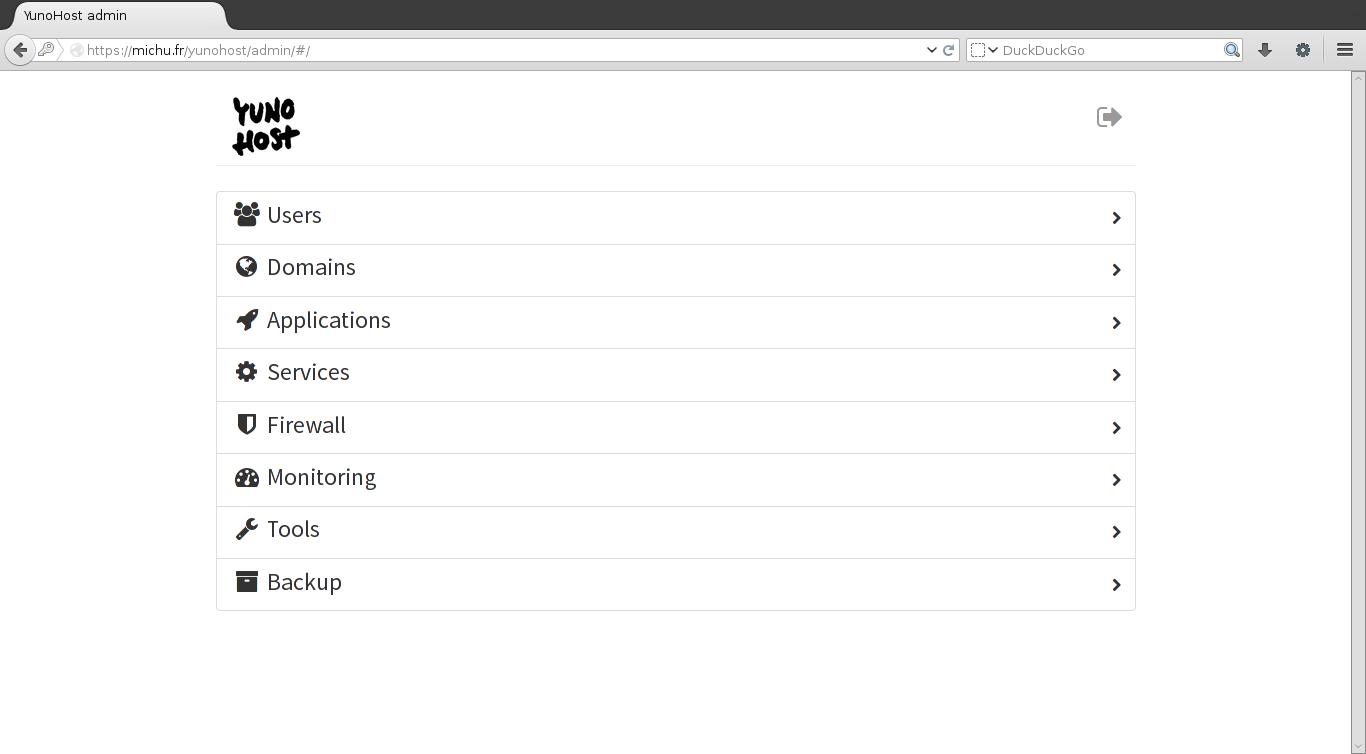
\includegraphics[width=\textwidth]{img2/17a-capture-yunohost.png}
\vfill
\end{center}
\end{frame}

\begin{frame}[t]
\begin{center}
\vfill
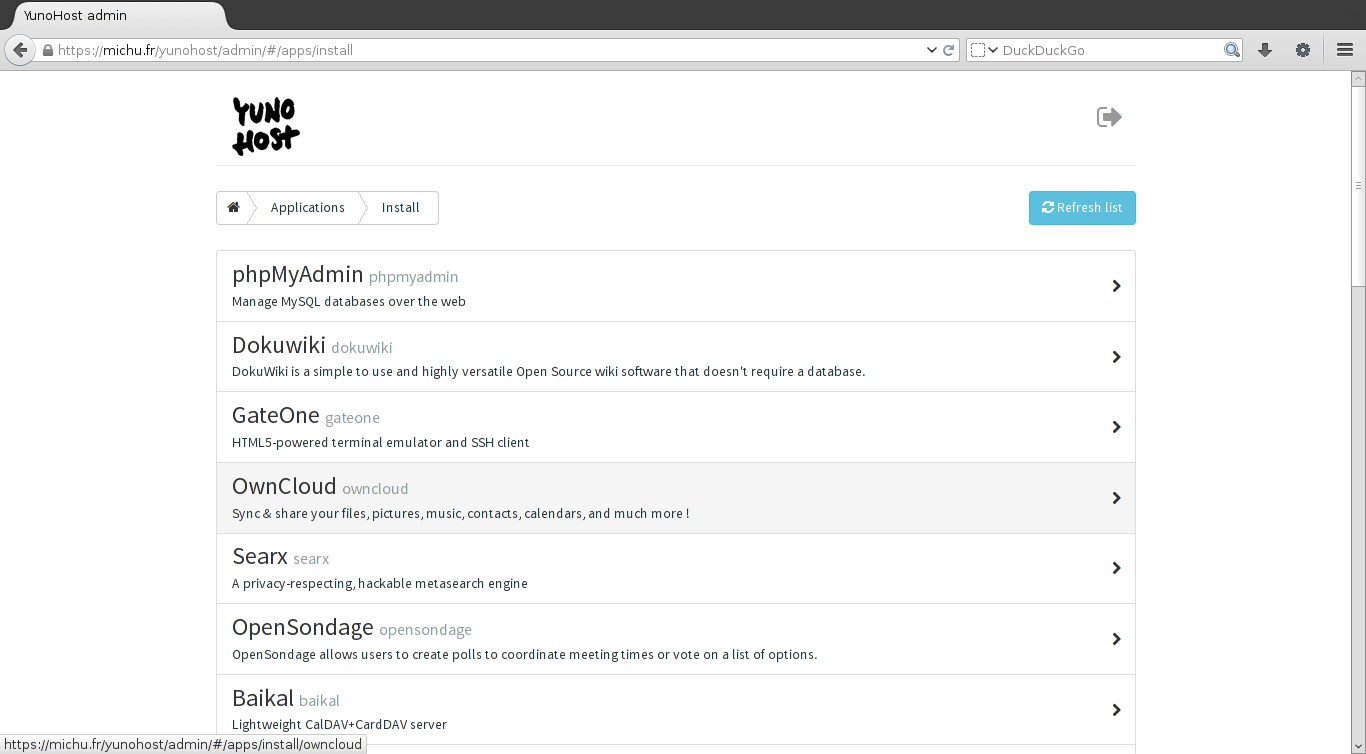
\includegraphics[width=\textwidth]{img2/19-capture-yunohostapps.png}
\vfill
\end{center}
\end{frame}

\begin{frame}[t,plain]
\begin{center}
\vspace{\fill}
	   \color{white}{\fontsize{60}{60}\selectfont Decentralized !}
	   \vspace{\fill}
\end{center}
\end{frame}


\begin{frame}[t]
\frametitle{\textcolor{titre}{Price ~?}}  \begin{center}

\includegraphics[width=.6\textwidth]{img2/Shut-up-and-take-my-money.jpg}
%
\includegraphics[width=0.4\textwidth]{img2/saco.png}
  \end{center}
\end{frame}

\begin{frame}[t]
\frametitle{\textcolor{titre}{Olimex board}}
  \begin{center}
    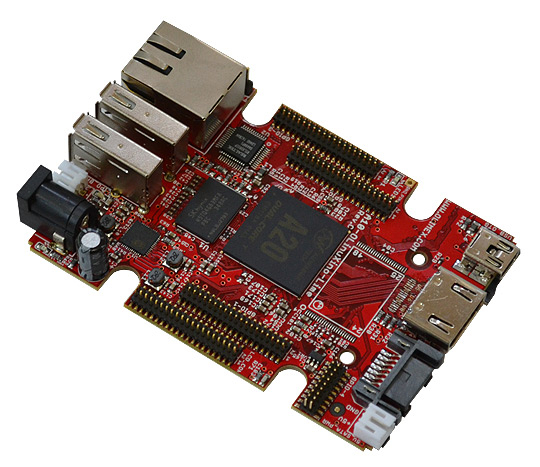
\includegraphics[width=0.7\textwidth]{img2/olimex.jpg}
  \end{center}
\end{frame}

\begin{frame}[t]
\frametitle{\textcolor{titre}{Box}}
  \begin{center}
    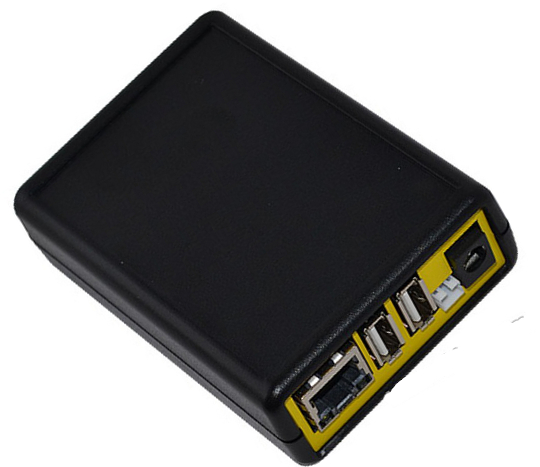
\includegraphics[width=0.7\textwidth]{img2/olimex-boite.jpg}
  \end{center}
\end{frame}
\begin{frame}[t]
\frametitle{\textcolor{titre}{Power supply}}
  \begin{center}
    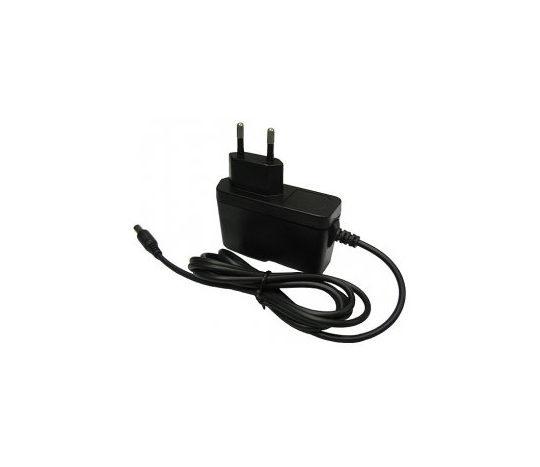
\includegraphics[width=0.7\textwidth]{img2/adaptateur.jpg}
  \end{center}
\end{frame}

\begin{frame}[t]
\frametitle{\textcolor{titre}{Wifi antenna}}
  \begin{center}
    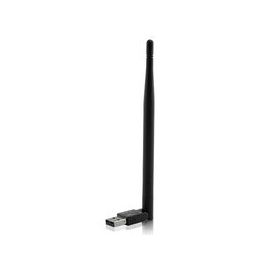
\includegraphics[width=0.6\textwidth]{img2/antenne.jpg}
  \end{center}
\end{frame}

\begin{frame}[t]
\frametitle{\textcolor{titre}{Memory card}}
  \begin{center}
    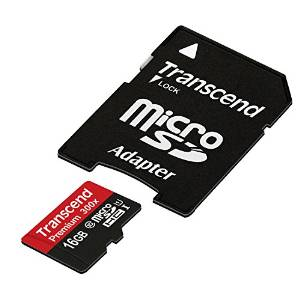
\includegraphics[width=0.6\textwidth]{img2/cartemem.jpg}
  \end{center}
\end{frame}

\begin{frame}[t]{}
\begin{center}
\vfill
\vfill{\Large Approximately \textbf{70\euro{} for 1 complete$^*$} Cube \\ 
(shipping costs included)}
\vspace{1cm}

{\Large Approximately \textbf{7 \euro{} / months} for a \\ \textbf{VPN}}
\vspace{1cm}
\vfill

{\footnotesize \emph{* for a grouped order > 9 Cubes, otherwise 80\euro{}}}
\vfill
\end{center}
\end{frame}

%\begin{frame}[t]
%\frametitle{\textcolor{titre}{I have a Cube !}}
%\begin{center}
%  \vfill
%    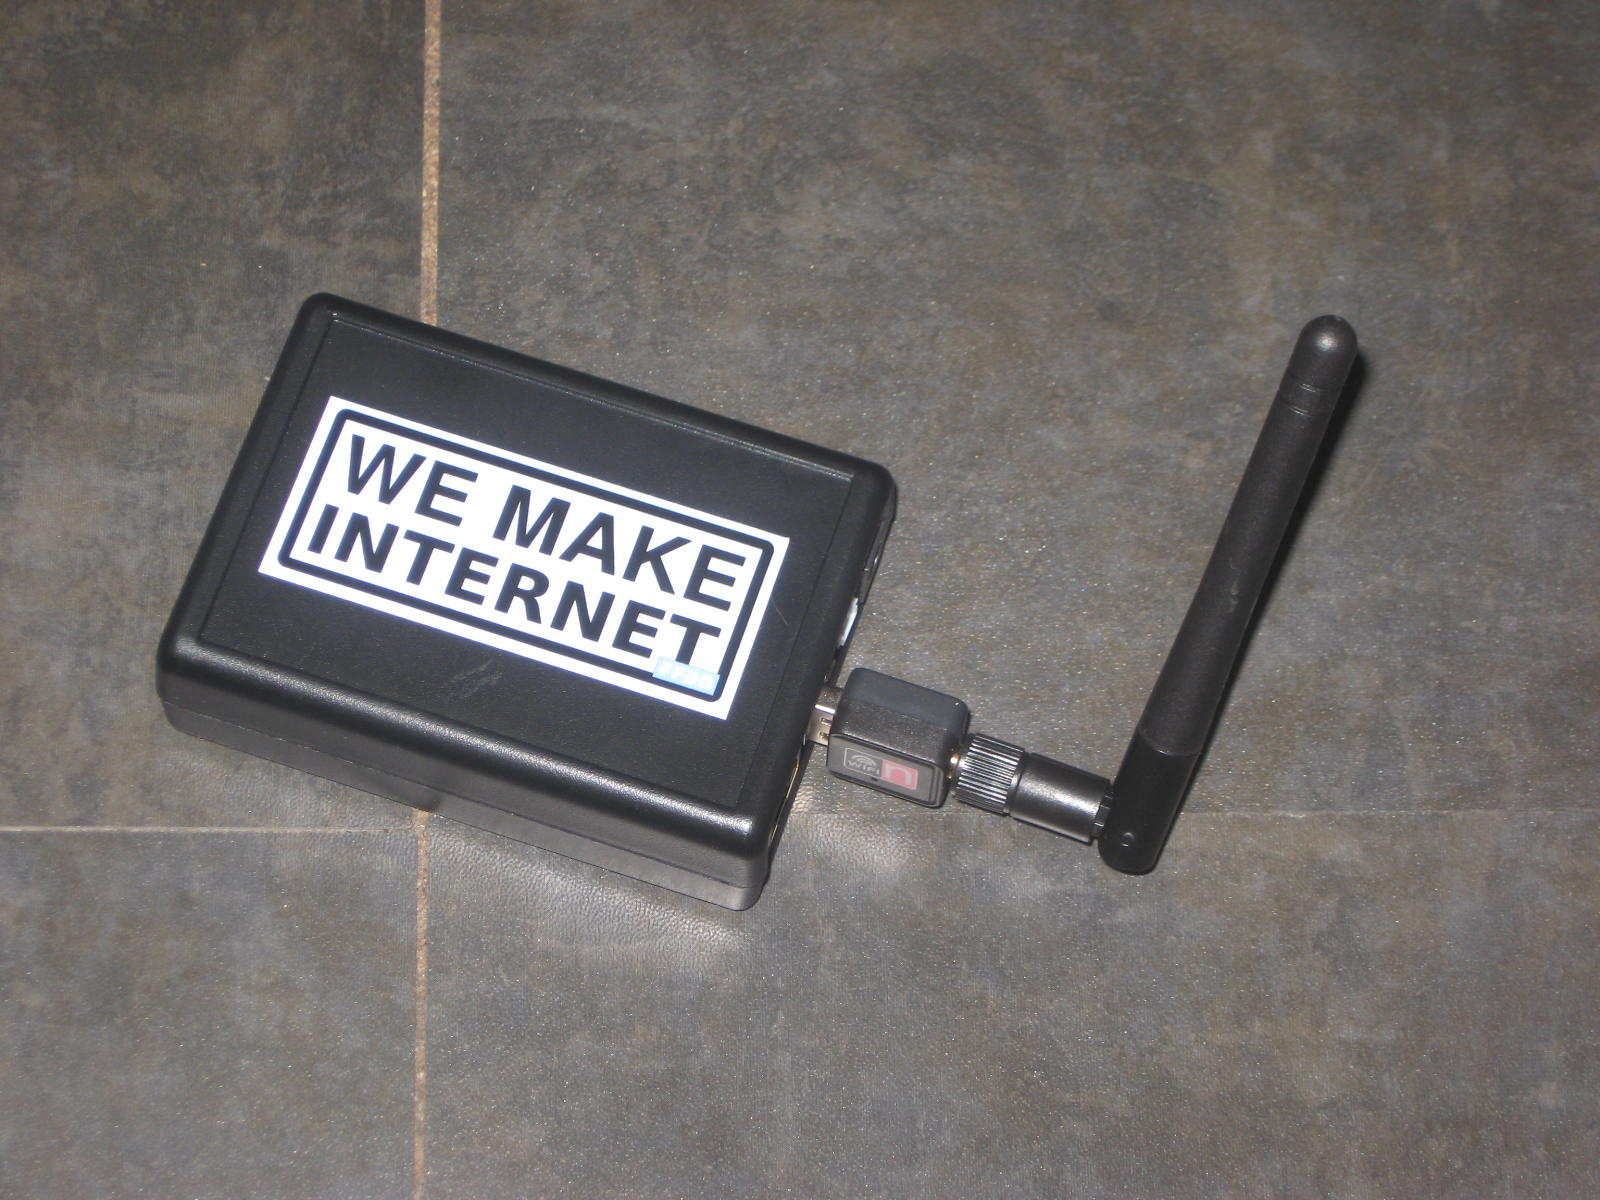
\includegraphics[width=.75\textwidth]{img2/04-photo-boitier.jpg}
%  \vfill
%\end{center}
%\end{frame}
%
%\begin{frame}[t]
%\frametitle{\textcolor{titre}{Connect the Cube to the ISP modem/router}}
%\begin{center}
%\vfill
%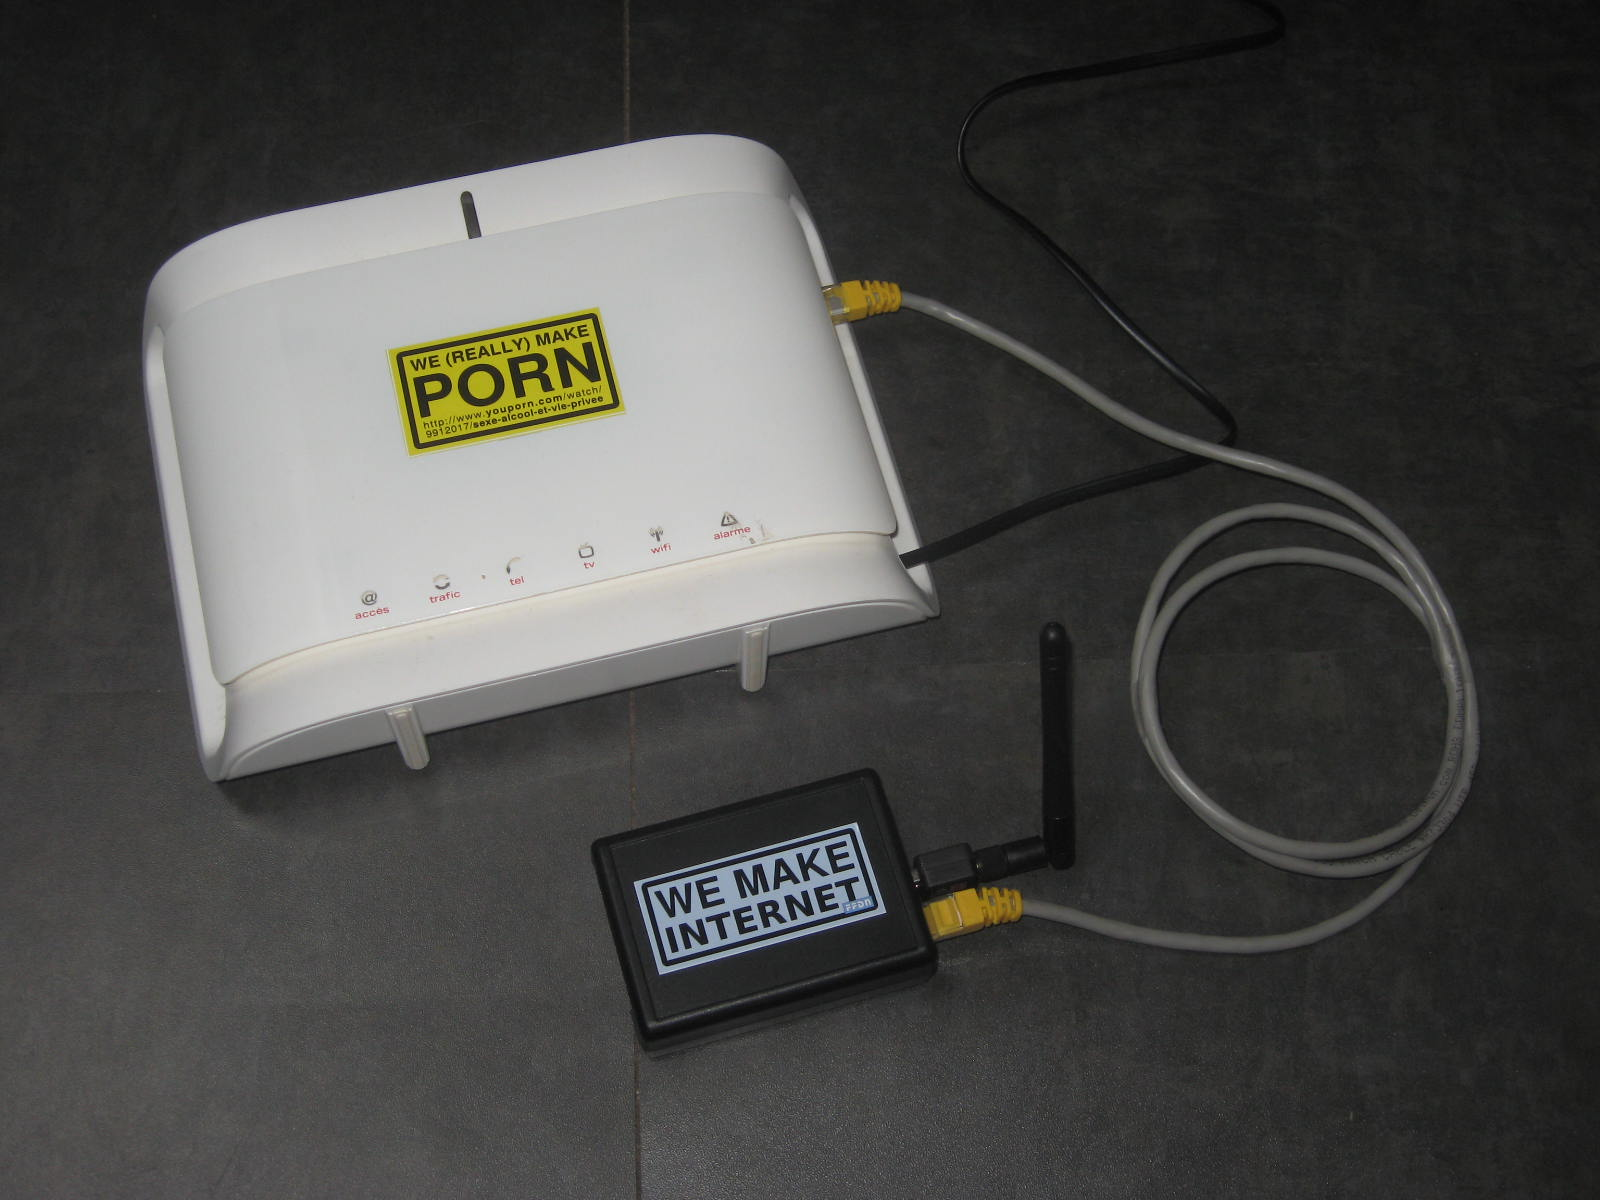
\includegraphics[width=.75\textwidth]{img2/05-photo-neufboxboitier.jpg}
%\vfill
%\end{center}
%\end{frame}
%
%\begin{frame}[t]
%\frametitle{\textcolor{titre}{It is space efficient}}
%\begin{center}
%\vfill
%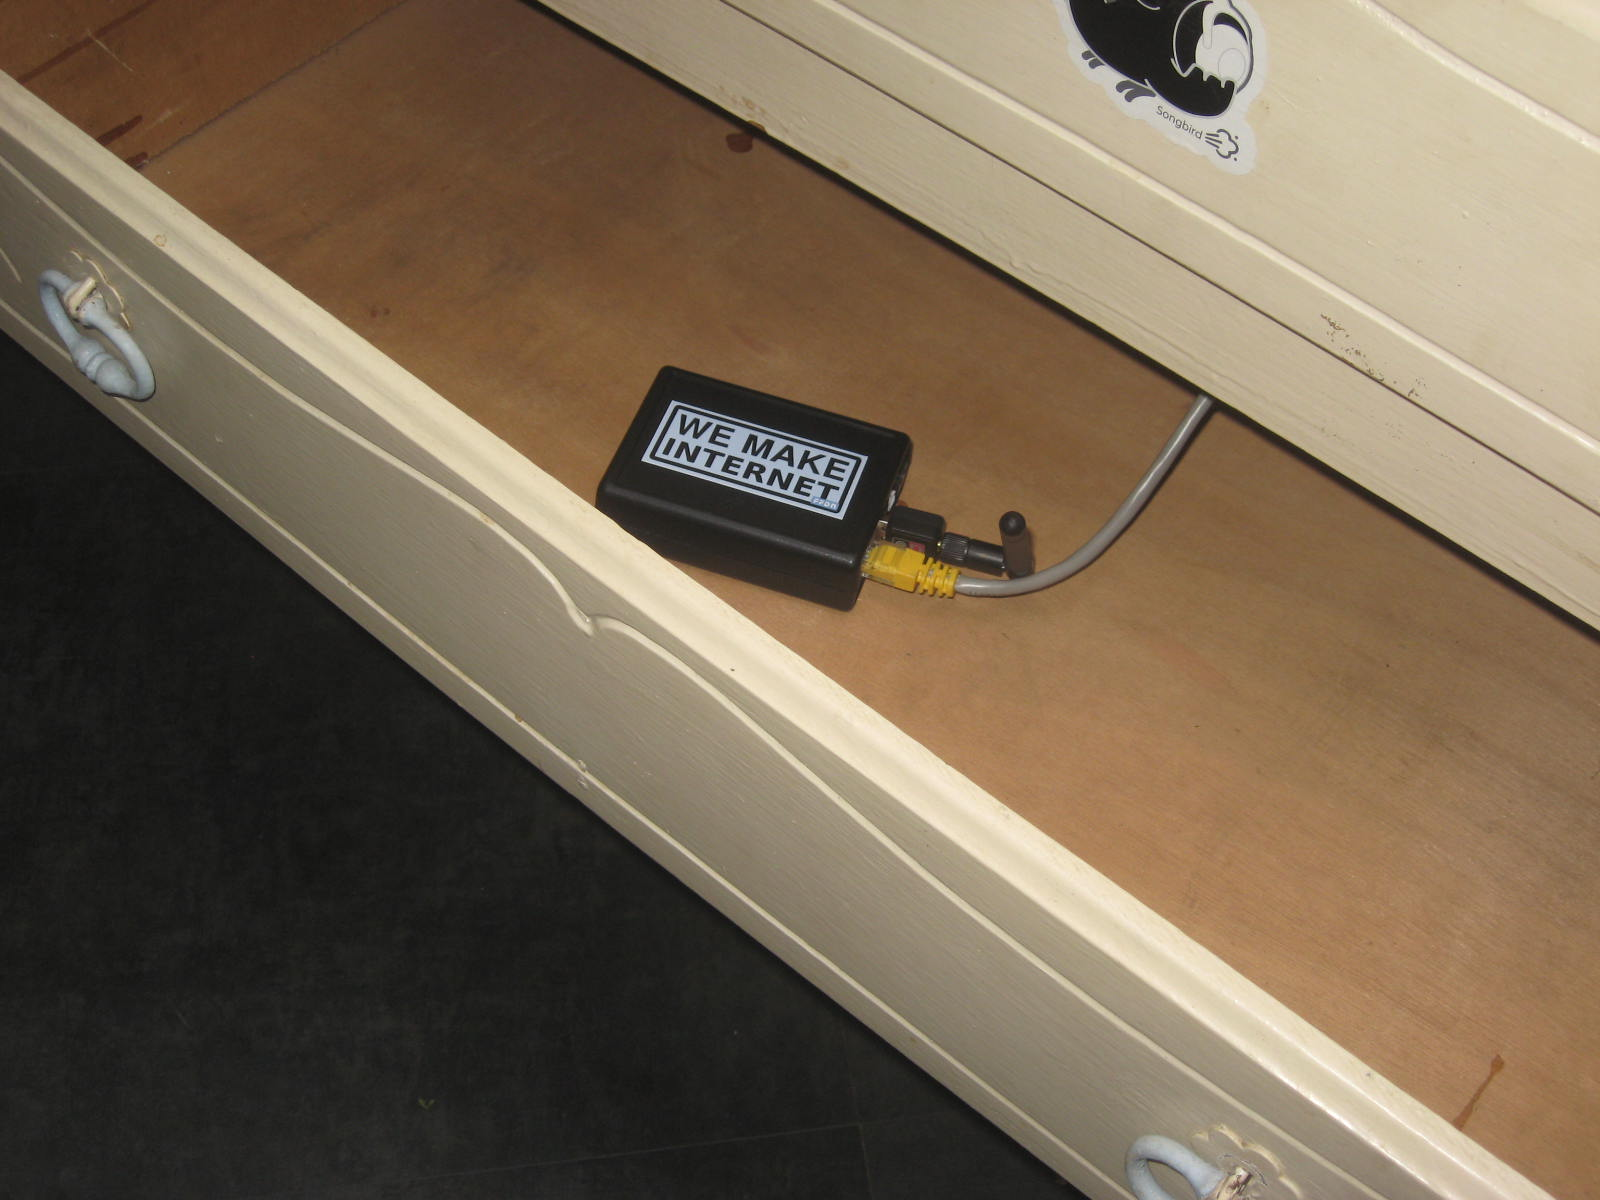
\includegraphics[width=.75\textwidth]{img2/16-photo-boitiercommode.jpg}
%\vfill
%\end{center}
%\end{frame}

\begin{frame}[t]
\frametitle{\textcolor{titre}{And it works out of the Cube}}
\begin{center}
\vfill
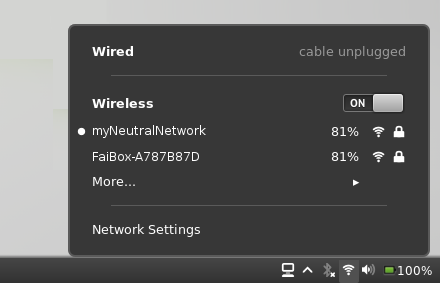
\includegraphics[width=.8\textwidth]{img2/06-capture-wifiboitier.png}
\vfill
\end{center}
\end{frame}

%\begin{frame}[t]
%\frametitle{\textcolor{titre}{I can still use the other services of my ISP
%(phone, TV)}}
%\begin{center}
%\vfill
%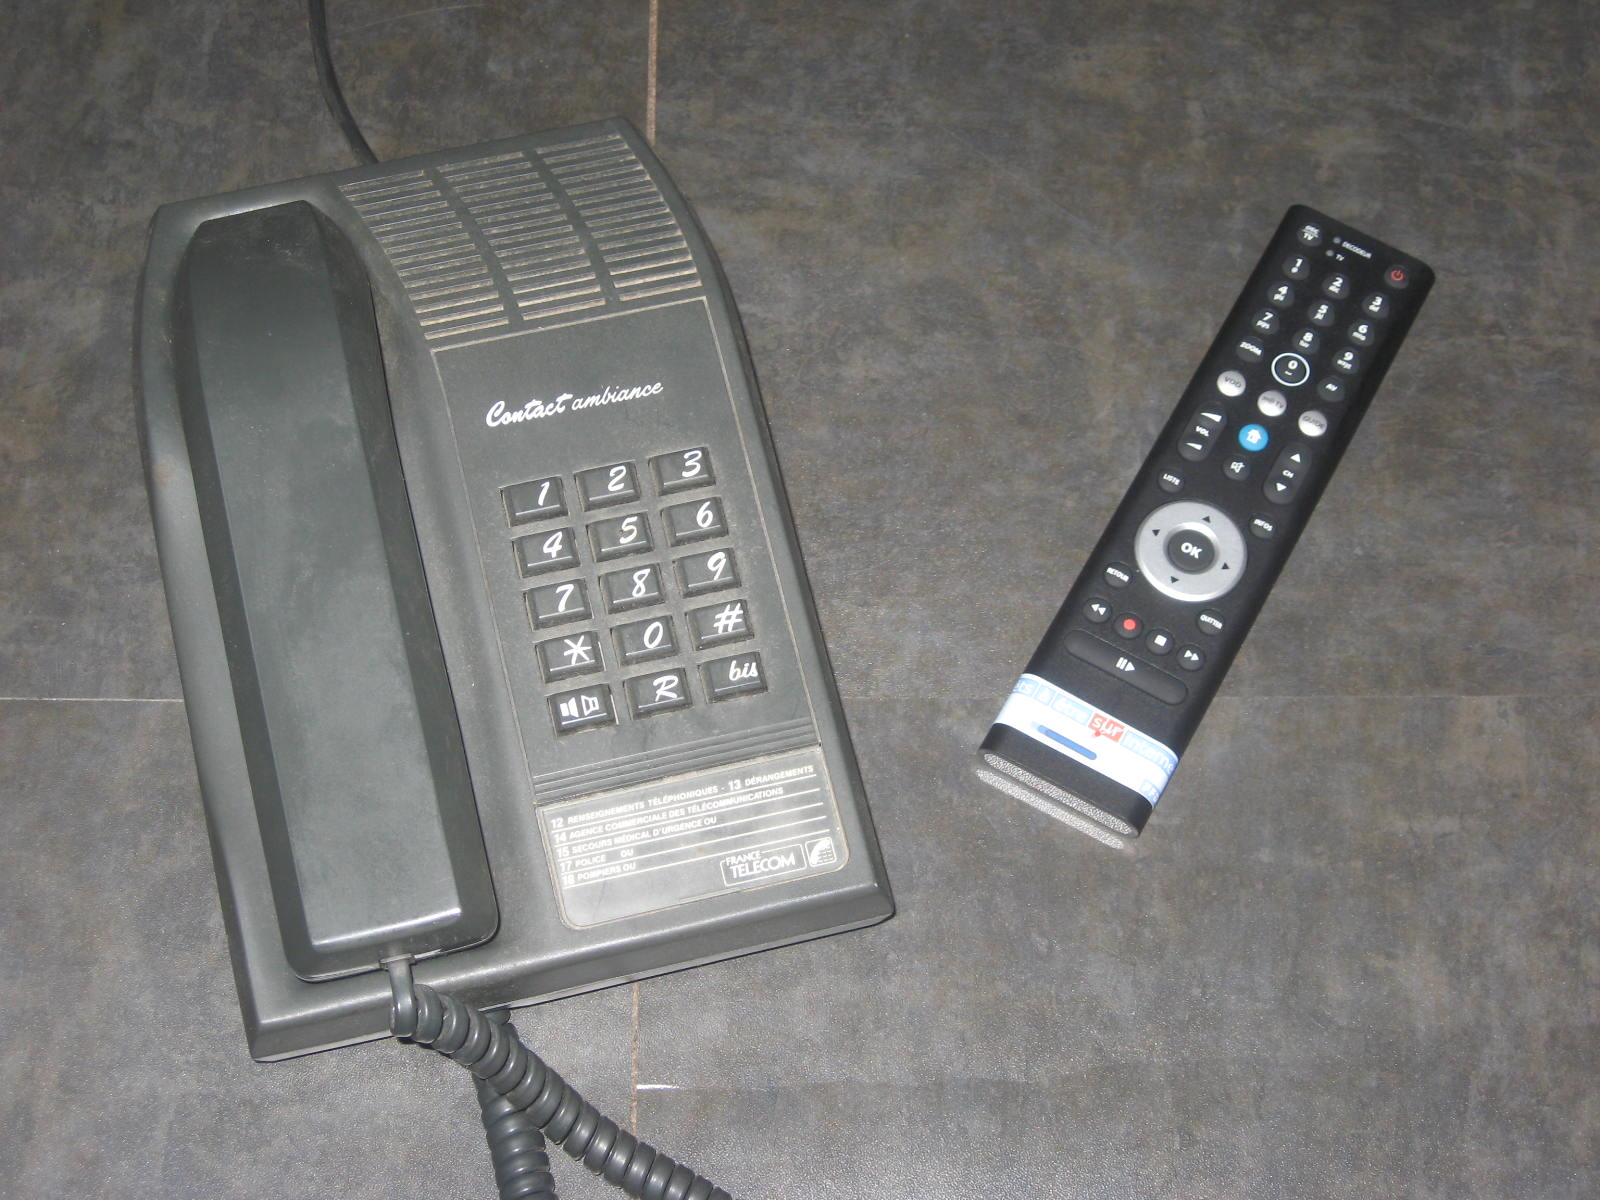
\includegraphics[width=.75\textwidth]{img2/13-photo-teltv.jpg}
%\vfill
%\end{center}
%\end{frame}

\begin{frame}[t]
\frametitle{\textcolor{titre}{Outline}}
  \begin{center}
    The Internet Cube enables you to :
    \vfill
    \begin{itemize}
      \item Easily \textbf{clean} your Internet access
      \item \textbf{self-host} services and personal data without huge computer skills
    \end{itemize}
    \end{center}
    \vfill
    %\pause And it's not over yet…
\end{frame}

\begin{frame}[t]{}
\begin{center}
\vfill{\Huge \textbf{Where can you find this Cube?}}
\vspace{.5cm}

{\large \emph{Because this Cube is not yet in Amazon catalog}}
\vfill
\end{center}
\end{frame}

\begin{frame}[t]
\frametitle{\textcolor{titre}{From your local non-profit ISP}}
\begin{center}
\vfill
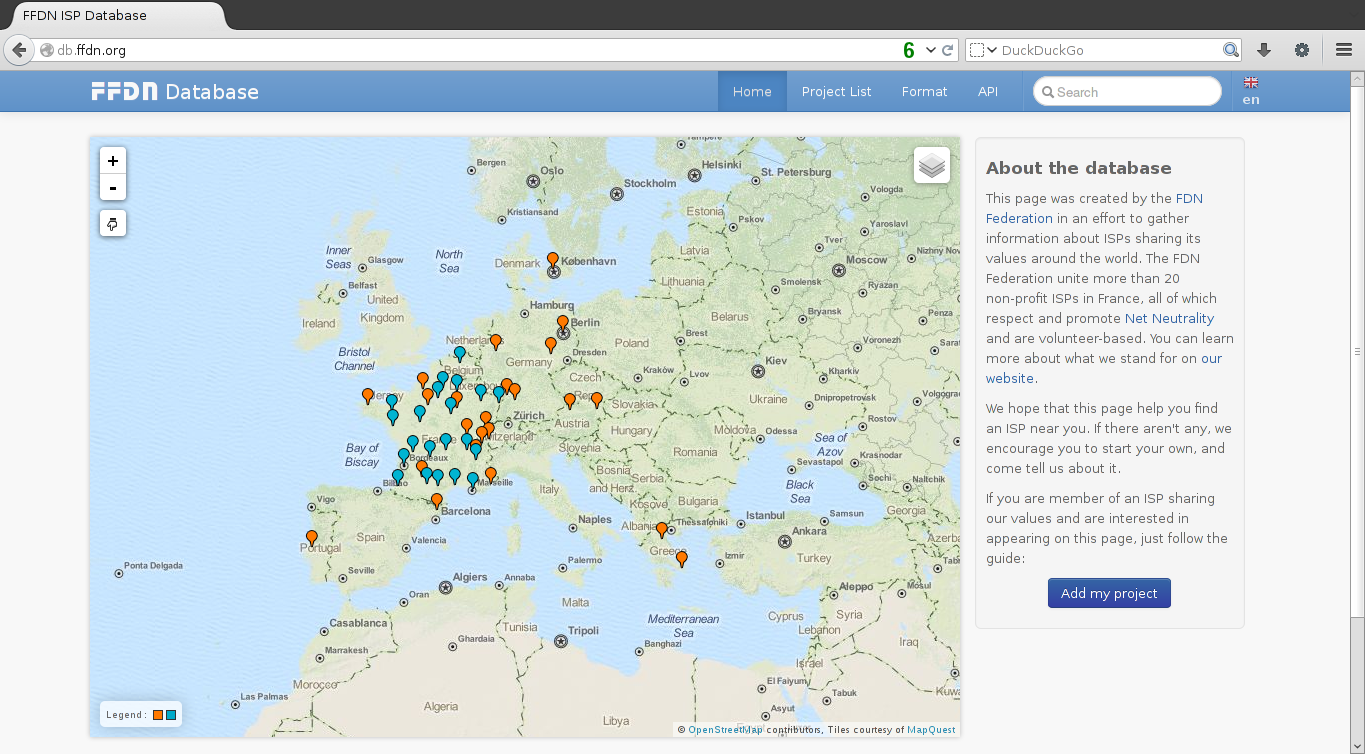
\includegraphics[width=\textwidth]{img2/25a-capture-ffdn.png}
\vfill
\end{center}
\end{frame}

\begin{frame}[t]
\frametitle{\textcolor{titre}{Or DIY because the software part is free}}
\begin{center}
\vfill
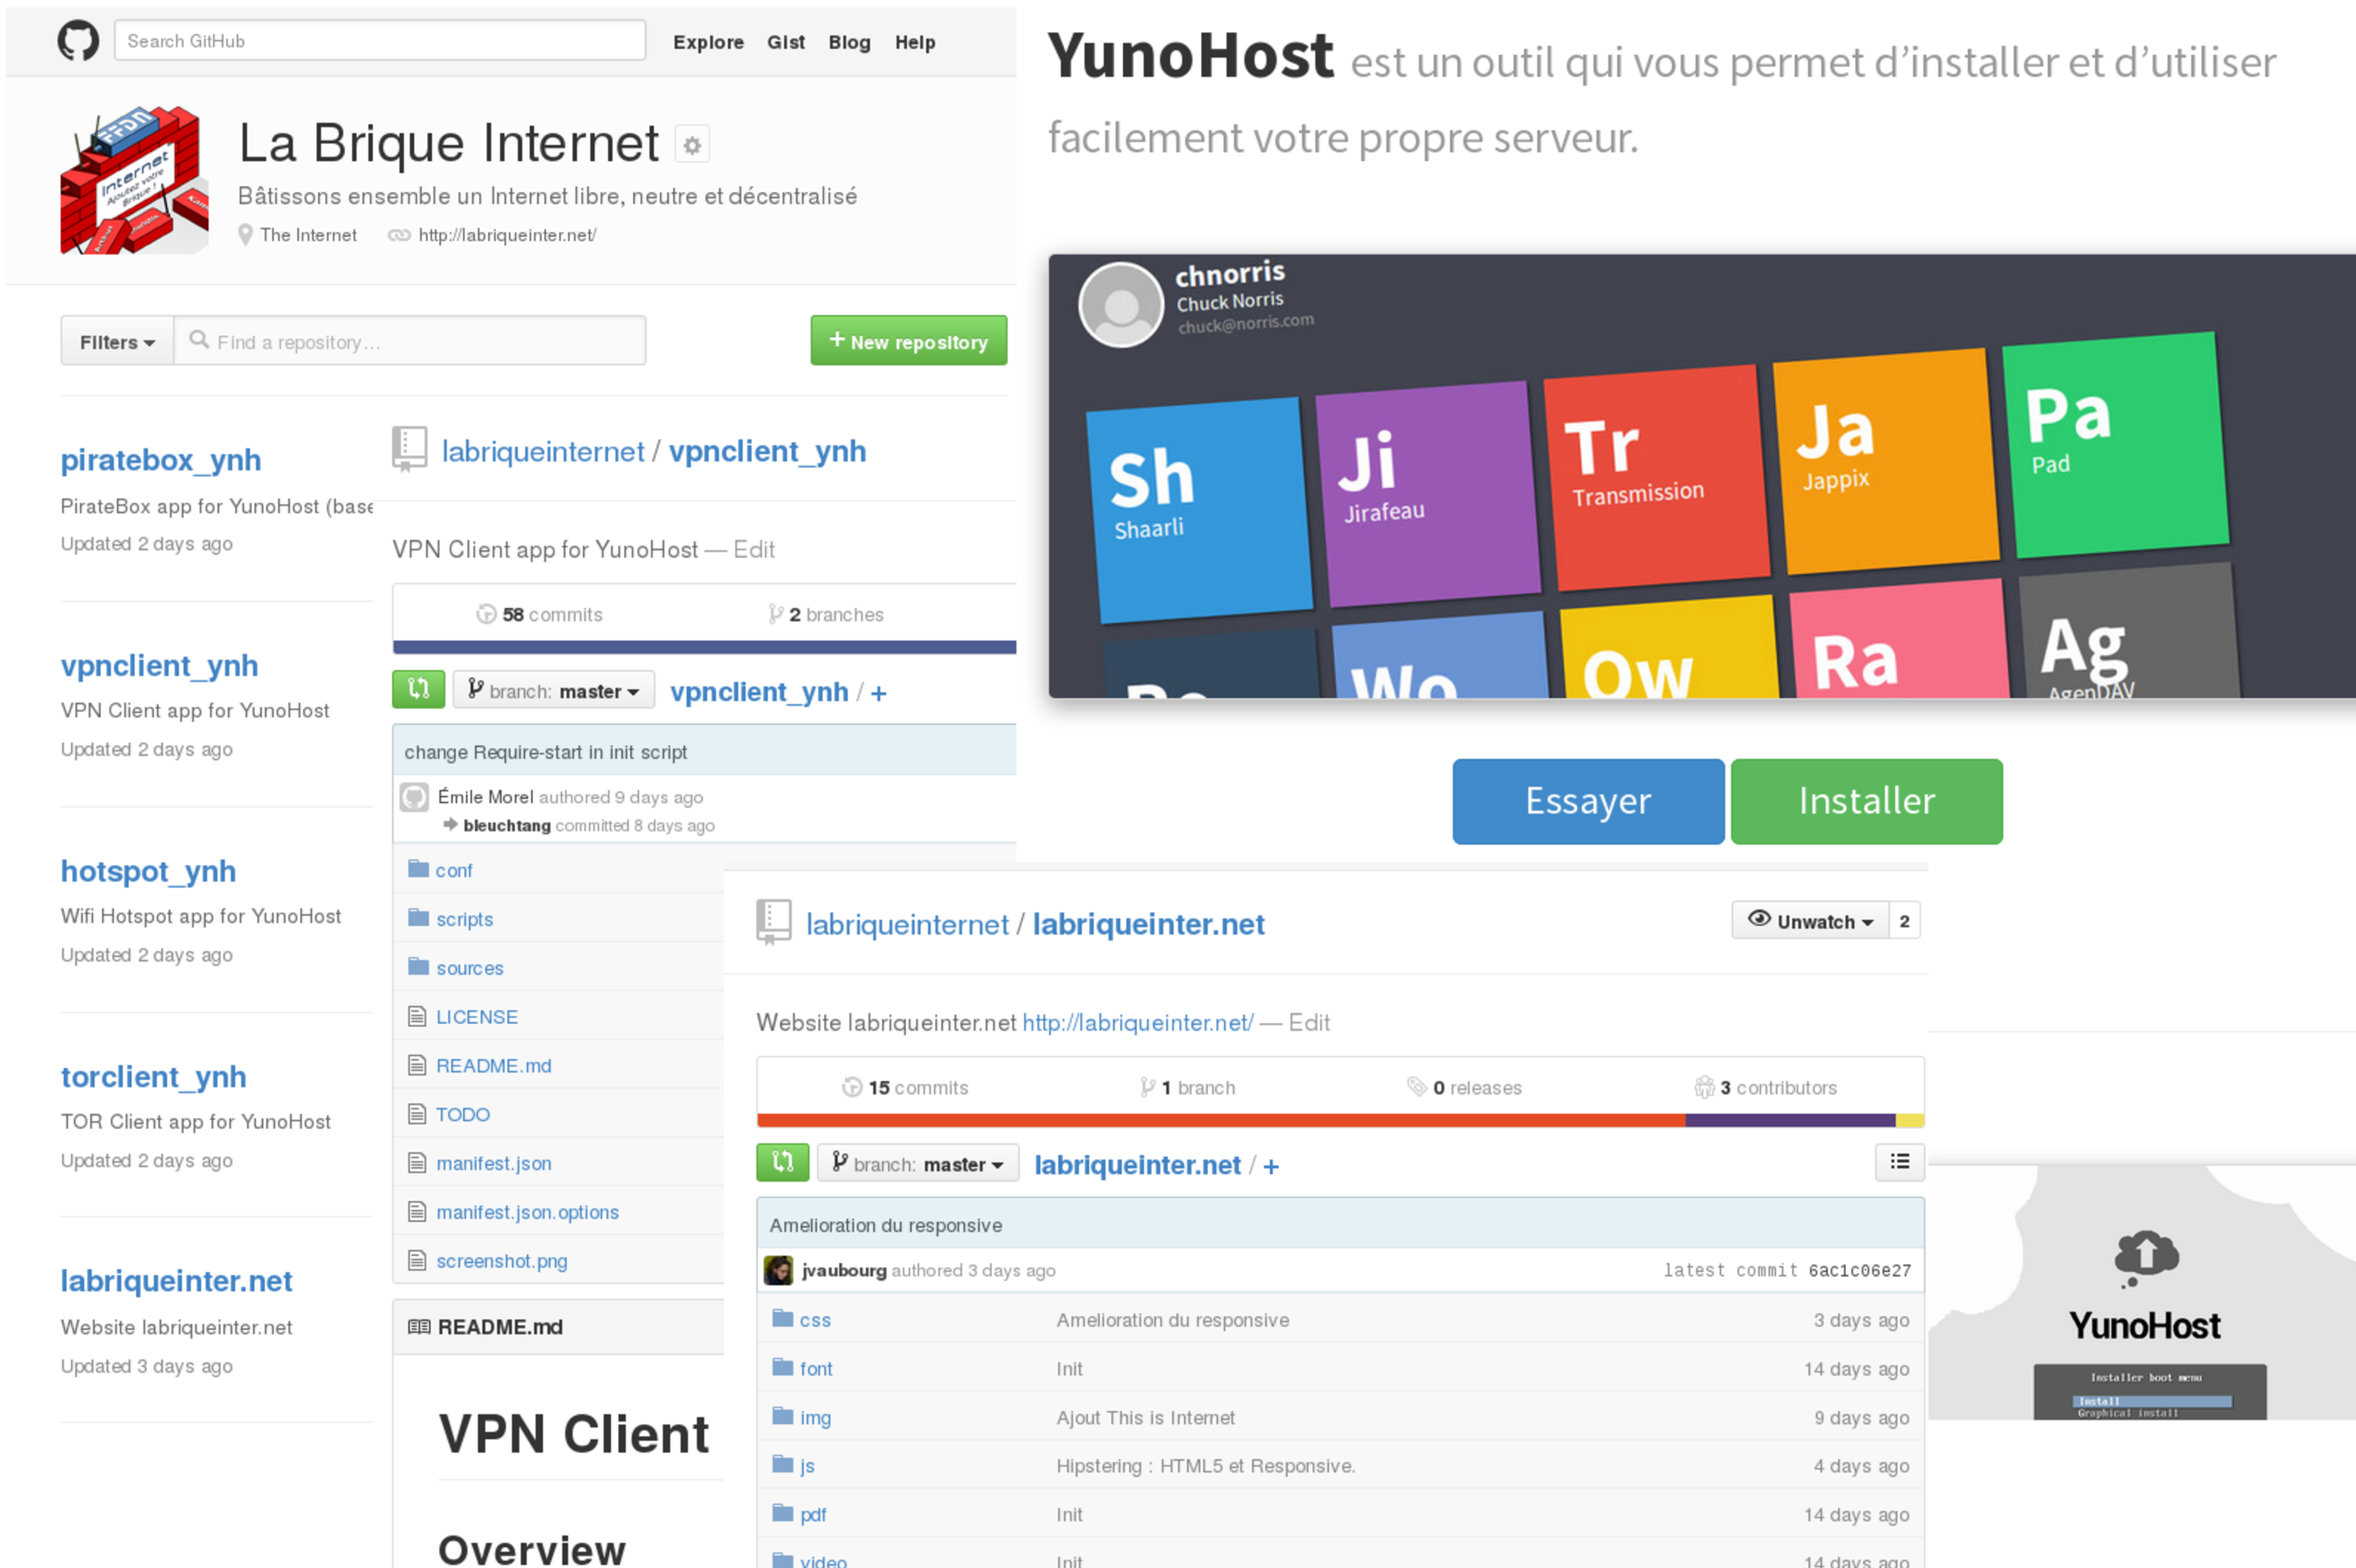
\includegraphics[width=10cm]{img2/25b-capture-github-contrib.pdf}
\vfill
\end{center}
\end{frame}

%\begin{frame}[t]
%\frametitle{\textcolor{titre}{And it's not finished…}}
%\vfill
%\begin{center}
%\begin{itemize}
%    \item Yunhost allows the self-hosting easily (jabber, mail, …)
%    \item Just move your Cube to
%    \begin{itemize}
%      \item having its services, and its data with you (holidays, relocation)
%      \item \textbf{to keep} its Internet access
%      \item \textbf{share} with others a clean Internet access (events)
%    \end{itemize}
%    \pause
%  \item Clean any Internet access (for example a 3G cell phone access)
%  \item Have fix and public \textbf{ipv4 and ipv6} addresses
%\end{itemize}
%\end{center}
%\end{frame}


%
%\begin{frame}[t]
%\frametitle{\textcolor{titre}{The Cube applications :}}
%\vfill
%\begin{center}
%\begin{itemize}
%    \item Neutral Internet connexion through a VPN
%\end{itemize}
%\end{center}
%\end{frame}
%
%\begin{frame}[t]
%\frametitle{\textcolor{titre}{The VPN Cube}}
%\vfill
%\begin{center}
%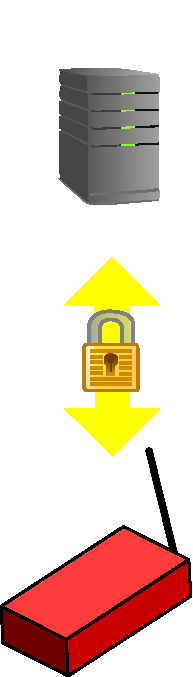
\includegraphics[scale=0.5]{img2/vpnen.pdf}
%\end{center}
%\end{frame}
%
%\begin{frame}[t]
%\frametitle{\textcolor{titre}{The Cube applications :}}
%\vfill
%\begin{center}
%\begin{itemize}
%    \item Neutral Internet connexion through a VPN
%    \item Share Box
%\end{itemize}
%\end{center}
%\end{frame}
%
%\begin{frame}[t]
%\frametitle{\textcolor{titre}{The VPN Cube}}
%\vfill
%\begin{center}
%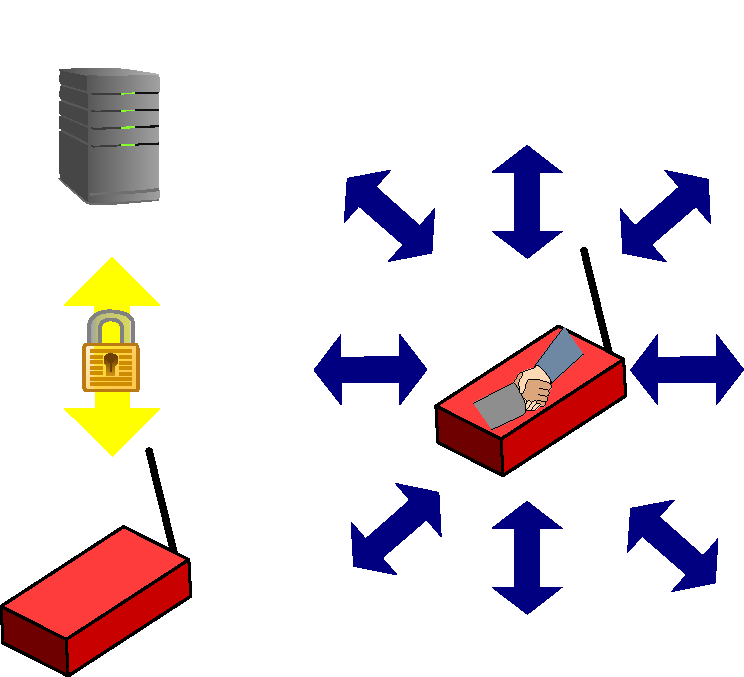
\includegraphics[scale=0.5]{img2/vpnpirateen.pdf}
%\end{center}
%\end{frame}
%
%\begin{frame}[t]
%\frametitle{\textcolor{titre}{The Cube applications :}}
%\vfill
%\begin{center}
%\begin{itemize}
%    \item Neutral Internet connexion through a VPN
%    \item Share Box
%    \item Tor Access
%\end{itemize}
%\end{center}
%\end{frame}
%
%\begin{frame}[t]
%\frametitle{\textcolor{titre}{The VPN Cube}}
%\vfill
%\begin{center}
%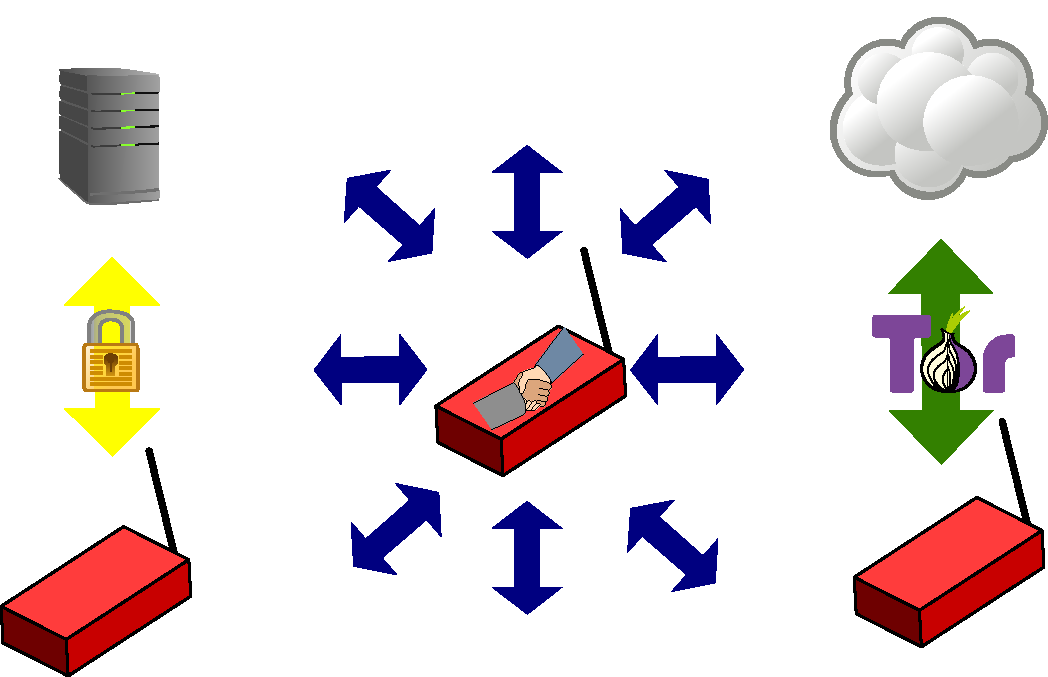
\includegraphics[scale=0.5]{img2/vpnpiratoren.pdf}
%\end{center}
%\end{frame}

\begin{frame}[t]
\frametitle{\textcolor{titre}{The Cube applications :}}
\vfill
\begin{center}
\begin{itemize}
    %\item Neutral Internet connexion through a VPN
    \item Pirate Box
    \item Tor Proxy \pause
	 %\item Three together (multi SSID) \good \pause
	 \item Clear your mobile Internet Access
	 \item Mediacenter 
	 \item Portable Mesh node
	 \item Temporary collaborative server 
	 \item Nas 
	 \item …
\end{itemize}
\end{center}
\end{frame}

%\begin{frame}[t]
%\frametitle{\textcolor{titre}{Next step, not so far}}
%\vfill
%\begin{center}
%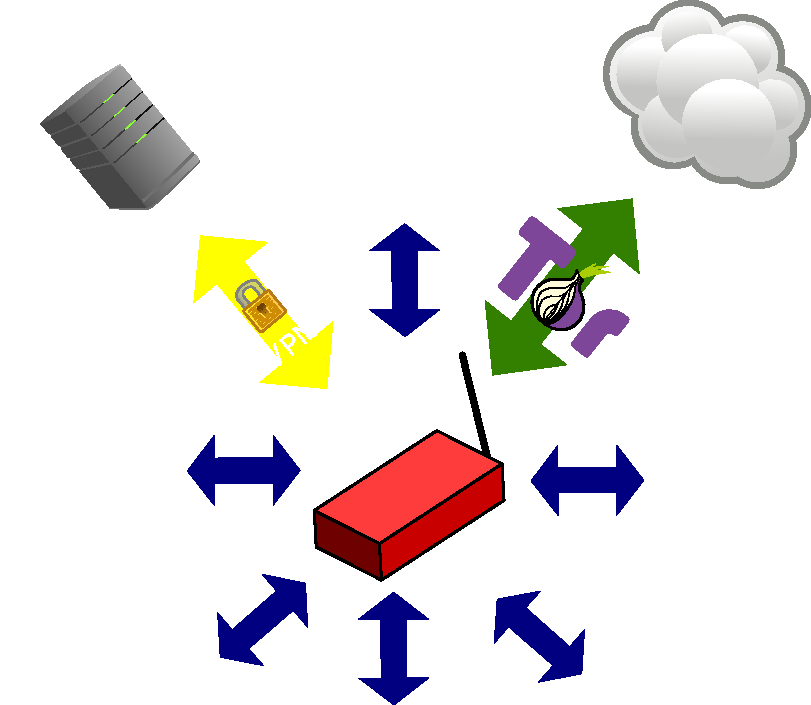
\includegraphics[scale=0.5]{img2/ultimateen.pdf}
%\end{center}
%\end{frame}

%\begin{frame}[t]
%\frametitle{\textcolor{titre}{The Internet Cube, is}}
%\vfill
%\begin{itemize}
%\item \textbf{free} yourself from the power of your ISP \vfill
%\item \textbf{regain} control of our services and data \vfill
%\item \textbf{use a clean Internet} peacefully
%\end{itemize}
%\vfill
%\end{frame}

%\begin{frame}[t]
%\frametitle{\textcolor{titre}{The Internet Cube ?}}
%\begin{center}
%\vfill
%
\includegraphics[width=.6\textwidth]{img2/Shut-up-and-take-my-money.jpg}
%\vfill
%\end{center}
%\end{frame}

\begin{frame}[t]
  \begin{center}
  \vfill
  \vspace{.5cm}{\Huge discussions@listes.labriqueinter.net}
  \vspace{1.5cm}
  \begin{itemize}
    \item Mailing Lists -- \url{https://listes.labriqueinter.net/}
    \item Images (beta) -- \url{https://repo.labriqueinter.net/}
    \item Build scripts -- \url{http://build.labriqueinter.net/}
  \end{itemize}
\vspace{.5cm}{\Huge \url{http://LaBriqueInter.net}}
%\\ To find an association near you : \vspace{.5cm} {\Large
%\url{http://db.ffdn.org}}

\end{center}
\end{frame}



\end{document}
